%\documentclass[12pt]{report}
%
%% some macros
%% Here, you can define your own macros. Some examples are given below.

\newcommand{\R}[0]{\mathds{R}} % real numbers
\newcommand{\Z}[0]{\mathds{Z}} % integers
\newcommand{\N}[0]{\mathds{N}} % natural numbers
\newcommand{\C}[0]{\mathds{C}} % complex numbers
\newcommand{\bm}[1]{{\boldsymbol{{#1}}}} % vector
\newcommand{\mat}[1]{{\boldsymbol{{#1}}}} % matrix

\newcommand{\E}[1]{\mathbb{E}_{#1}} % Expectation
\newcommand{\Pd}[1]{\mathbb{P}_{#1}} % Probability Distribution

%%%%%%%%%%%%%%%%%%%%%%%%%%%%%%%%%%%%%%%%%%
% University Assignment Title Page 
% LaTeX Template
% Version 1.0 (27/12/12)
%
% This template has been downloaded from:
%%%%%%%%%%%%%%%%%%%%%%%%%%%%%%%%%%%%%%%%%
%----------------------------------------------------------------------------------------
%	PACKAGES AND OTHER DOCUMENT CONFIGURATIONS
%----------------------------------------------------------------------------------------

\usepackage[nottoc,notlot,notlof]{tocbibind}
\usepackage[T1]{fontenc}
%\usepackage{hyperref}
\usepackage{indentfirst}
\usepackage{amsmath}
\usepackage{amssymb}
\usepackage{graphicx}
\usepackage{subcaption}
\usepackage{geometry}
 \geometry
 {
     a4paper,
     left=25mm,
     right=25mm,
     top=30mm,
     bottom=30mm,
 }

% \usepackage[a4paper,hmargin=2.8cm,vmargin=2.0cm,includeheadfoot]{geometry}
\usepackage{textpos}
\usepackage{natbib} % for bibliography
%\usepackage{tabularx,longtable,multirow,subfigure,caption}
\usepackage{fncylab} %formatting of labels
\usepackage{fancyhdr} % page layout
\usepackage{url} % URLs
\usepackage[english]{babel}
%\usepackage{dsfont}
\usepackage{epstopdf}
\usepackage{backref} % needed for citations
\usepackage{array}
\usepackage{latexsym}
\usepackage[pdftex,pagebackref,hypertexnames=false,colorlinks]{hyperref} % provide links in pdf
 
\hypersetup{pdftitle={},
  pdfsubject={}, 
  pdfauthor={},
  pdfkeywords={}, 
  pdfstartview=FitH,
  pdfpagemode={UseOutlines},% None, FullScreen, UseOutlines
  bookmarksnumbered=true, bookmarksopen=true, colorlinks,
    citecolor=black,%
    filecolor=black,%
    linkcolor=black,%
    urlcolor=black}
 
\usepackage[all]{hypcap}
\frenchspacing

\DeclareMathOperator{\tr}{tr}
%
%\begin{document}

\chapter{3D Facial Modelling Background}

This chapter shall discuss the preliminary background theory on 3D Facial Modelling and how this data is processed and represented for use with Deep Learning models.
In order to avoid representing data as a high dimensional point cloud, a lower dimensional representation of relevant variation in the data can be expressed with Blendshapes, found with Principal Component Analysis (PCA).
Data preprocessing involves bringing the data samples into correspondence (also referred to as alignment or registration) to remove undesirable variations in the data, this can be achieved with Procrustes Analysis.

\section{Data Collection and Representation}
Unlike 2D video where the subject is captured from a single angle without any depth information, 3D models cannot be captured with a single camera.
In most instances, 3D head scans are captured with the use of a multi-camera rig with multiple cameras capturing video simultaneously.
The number and type of cameras can vary from system to system, but the principle remains consistent.
All cameras must be synchronised to capture footage at the same time, with the same frame rate.
This is inherently a more complex system than 2D video capture as is therefore more expensive, limiting the accessibility of such systems.  
Once the images have been captured, the footage must be combined in order to produce a 3D model of the subjects head \cite{Li2017}, often referred to as a facial mesh.
A facial mesh is made up of a point cloud of vertices and vertex connections.
Depending on the resolution of the system used to capture the data, the number of points which are used to represent the subject can vary, each with $x$, $y$ and $z$ coordinates in space.
Depending on the mesh capture pipeline, the number of vertices may vary, but even a low resolution mesh may contain several thousand vertices.
In the example shown in Figure \ref{fig:FLAME_Point_Cloud}, the FLAME model \cite{Li2017} uses around 5000 vertex positions, each with an $(x, y, z)$ value, resulting in a total number of 15,000 parameters for a single capture in time.
While Deep Learning models have been trained to drive all vertex positions from a starting template mesh \cite{Karras2017a}, a simpler representation can be achieved with the use of Blendshapes.

\begin{figure}[h]
    \centering
    \begin{subfigure}[b]{0.22\textwidth}
        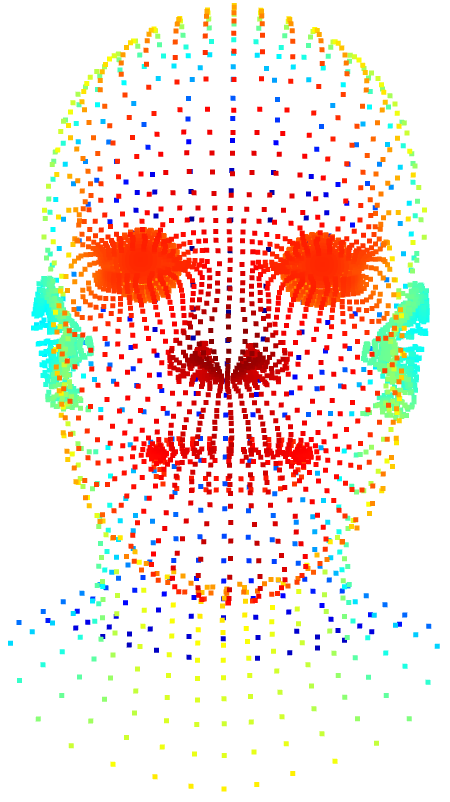
\includegraphics[width=\textwidth]{figures/flame_front.png}
    \end{subfigure}
    \hfill
    \begin{subfigure}[b]{0.31\textwidth}
        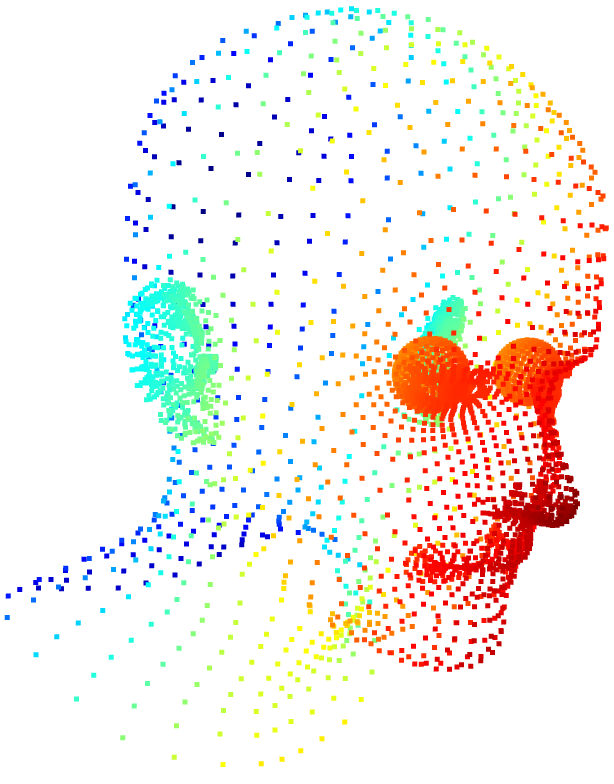
\includegraphics[width=\textwidth]{figures/flame_angle.png}
    \end{subfigure}
    \hfill
    \begin{subfigure}[b]{0.28\textwidth}
        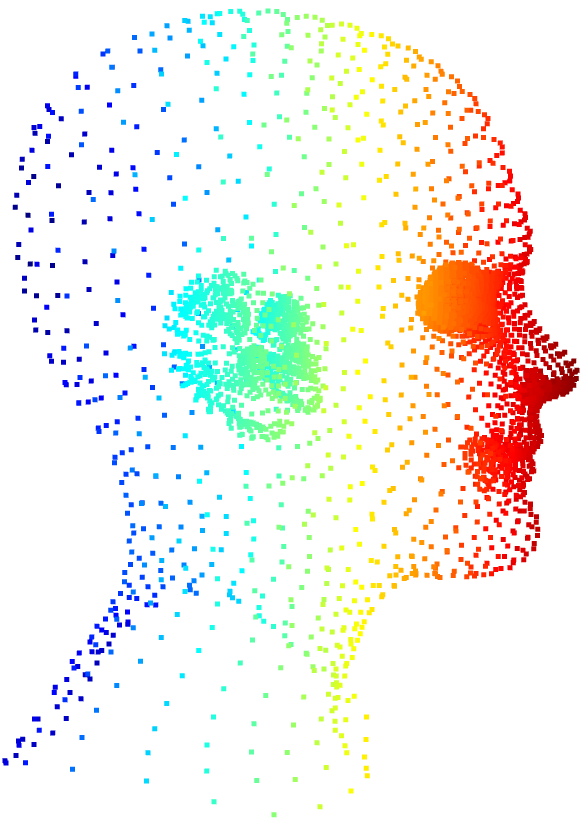
\includegraphics[width=\textwidth]{figures/flame_side.png}
    \end{subfigure}
    \caption{Point Cloud Representation of FLAME Model \cite{Li2017}}\label{fig:FLAME_Point_Cloud}
\end{figure}

\subsection{Blendshapes} \label{blendshapes}
Capturing realistic facial motion by modelling the displacements of all of these vertices is impractical when manipulating a model by hand and may hinder the performance of a Machine Learning model due to the high dimensionality of the data.
Blendshapes attempt to model aspects of realistic facial motion by finding the relations between these vertices and manipulating them simultaneously \cite{Lewis2010}, by reducing the number of parameters, the model becomes more manageable to control.
One method of producing model blendshapes is with the use of Principle Component Analysis (PCA).
By applying PCA on a dataset of facial meshes, the resulting principle components represent the changes in facial motion which capture the largest amount of variation in the set while reducing the number of model parameters substantially.

\subsubsection{Principal Component Analysis} \label{sec:pca}
Given a collection of measured data points in a high dimensional space, it is often desirable to reduce the dimensionality of such data to a lower dimensional latent space, this could be to aid processing the data or enable visualisation.
In such instances, it is desirable for the mapping to the latent space to maintain as much information from the original data as possible.

PCA aims to reduce the dimensionality of a collection of data points while maximising the variance in the latent space.
Alternatively, PCA aims to find a mapping from the original data to a new latent space which allow for the original data to be reconstructed with minimal error.
These two aims are in fact equivalent.

Let $\bm{x_i} \in \mathbb{R}^f$ represent a data point in $f$ dimensional space and $\bm{y_i} \in \mathbb{R}^d$ represent the point which $\bm{x_i}$ is transformed to by a linear transformation $\mat{W}$ equation (\ref{eq:pca_transformation}), where $d << f$.

\begin{equation} \label{eq:pca_transformation}
    \bm{y_i} = \mat{W}^\top \bm{x_i}
\end{equation}
where,

\begin{equation*}
    \bm{y_i} = \begin{bmatrix} 
                y_{i1} \\
                \vdots \\
                y_{id} 
               \end{bmatrix},
    \quad
    \bm{x_i} = \begin{bmatrix} 
                \bm{x}_{i1} \\
                \vdots \\
                \bm{x}_{if} 
               \end{bmatrix},
    \quad
    \mat{W} = [
               \bm{w_1}, \dots, \bm{w_d}
              ],
    \quad
    \bm{w_i} = \begin{bmatrix} 
                w_{i1} \\
                \vdots \\
                w_{if} 
               \end{bmatrix}
\end{equation*}

\bigskip
The optimal transformation $\mat{W}$ will maximise the variance in the data, where variance is expressed by equation (\ref{eq:variance}).
This then follows that the optimal solution is found by maximising equation (\ref{eq:pca_optimum_transformation}).
To prevent the trivial solution where $\bm{w}_k = \infty$, constrain a fixed magnitude $\mat{W}^\top \mat{W} = \mat{I}$.


\begin{equation} \label{eq:variance}
    \sigma_y^2 = \frac{1}{N} \sum_{i=1}^{N} (y_{ik} - \mu_k)^2
\end{equation}
where,
\begin{equation*}
    \mu_k = \frac{1}{N} \sum_{i=1}^N y_{ik}
\end{equation*}

\begin{align*}
    \mat{W} &=\operatorname*{arg}\operatorname*{max}_\mat{W} 
                \frac{1}{N} \sum_{k=1}^{d} \sum_{i=1}^{N} 
                (y_{ik} - \mu_k)^2 \\
            &=\operatorname*{arg}\operatorname*{max}_\mat{W} 
                \frac{1}{N} \sum_{k=1}^{d} \sum_{i=1}^{N} 
                \bm{w}_k^\top 
                (\bm{x}_i - \bm{\mu})
                (\bm{x}_i - \bm{\mu})^\top 
                \bm{w}_k \\
            &=\operatorname*{arg}\operatorname*{max}_\mat{W} 
                \sum_{k=1}^{d}
                \bm{w}_k^\top 
                \mat{S}_t
                \bm{w}_k \\
\end{align*}
where $\mat{S}_t$ is the covariance matrix,
\begin{equation} \label{eq:covariance}
    \mat{S}_t = \frac{1}{N} \sum_{i=1}^{N} 
                (\bm{x}_i - \bm{\mu})
                (\bm{x}_i - \bm{\mu})^\top 
\end{equation}
and,
\begin{equation*}
    \bm{\mu} = \frac{1}{N} \sum_{i=1}^N \bm{x}_i
\end{equation*}


\begin{equation} \label{eq:pca_optimum_transformation}
    \mat{W} = \operatorname*{arg}\operatorname*{max}_\mat{W} 
          \tr[\mat{W}^\top \mat{S}_t \mat{W}],
          \quad
    \text{subject to} \quad 
    \mat{W}^\top \mat{W} = \mat{I}
\end{equation}

\bigskip
By constructing the Lagrangian from equation (\ref{eq:pca_optimum_transformation}) and solving the solution in equation (\ref{eq:pca_solved}) can be obtained.
From eigendecomposition, $\mat{W}$ has columns of eigenvectors which correspond to the $d$ largest non-zero eigenvalues of the covariance matrix, $\mat{S}_t$.

\begin{equation*}
    L(\mat{W}, \mat{\Lambda}) = \tr[\mat{W}^\top \mat{S}_t \mat{W}] - \tr[\Lambda(\mat{W}^\top \mat{W} - \mat{I})]
\end{equation*}

\begin{equation*}
    \frac{\partial \tr[\mat{W}^\top \mat{S}_t \mat{W}]}{\partial \mat{W}} = 2 \mat{S}_t \mat{W},
    \quad
    \frac{\partial \tr[\Lambda(\mat{W}^\top \mat{W} - \mat{I})]}{\partial \mat{W}} = 2 \mat{W \Lambda}
\end{equation*}

\begin{equation*}
    L(\mat{W}, \mat{\Lambda}) = 0 
\end{equation*}

\begin{equation} \label{eq:pca_solved}
    \mat{S}_t \mat{W} = \mat{W \Lambda}
\end{equation}

\section{Facial Mesh Alignment}
In order to create blendshapes from 3D facial scans, movement within scans should be limited to facial movement with as little head movement as possible.
If head movement remains within the scans, then this will be reflected in the principal axis produced by Principle Components Analysis (PCA) and as head motion is independent from speech, this is undesirable.
Initial data capture can aim to minimise subject head movement, however this cannot be completely eliminated.
To remove head motion from the dataset, the scans can be brought into alignment relative to landmark positions on the face which do not move during speech.
Such landmarks include the nose, corners of the eyes and cheek bones, as these points will be stationary during speech.
By aligning the meshes based on the variation in these points, the head position of the subjects can be constrained while the mouths are not.
To achieve this, Procrustes Analysis can be used.

\begin{figure}[h]
    \centering
    \begin{subfigure}[b]{0.4\textwidth}
        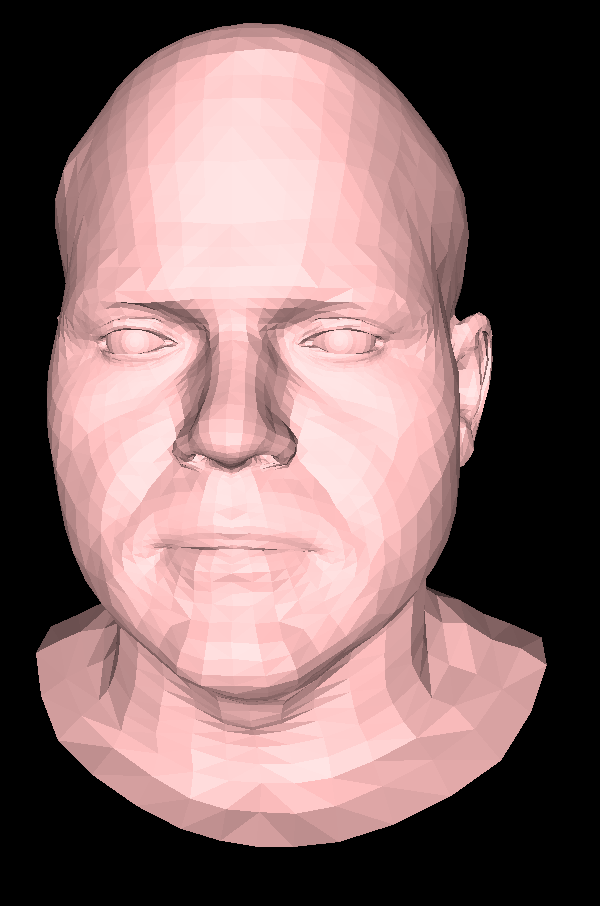
\includegraphics[width=\textwidth]{figures/subject2_unaligned.png}
    \end{subfigure}
    \begin{subfigure}[b]{0.4\textwidth}
        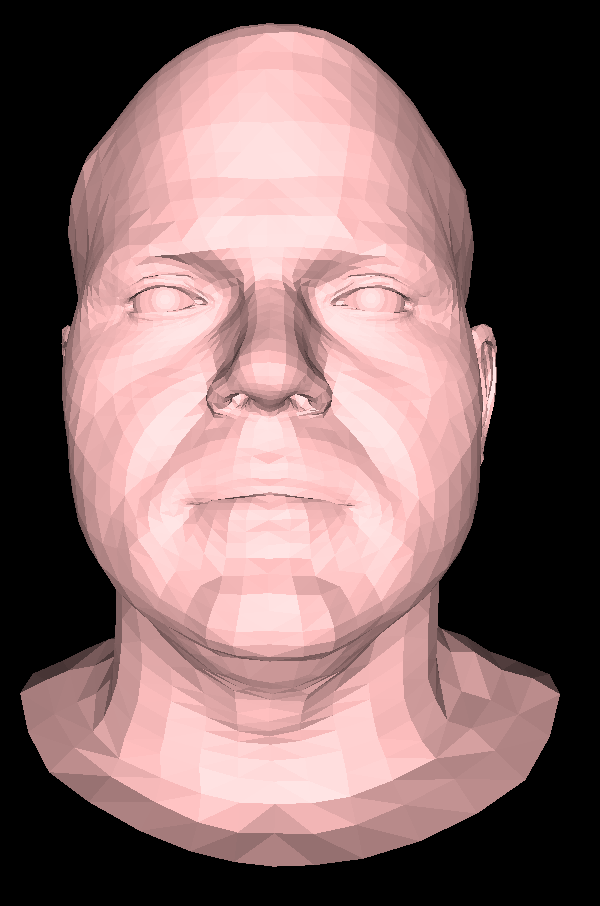
\includegraphics[width=\textwidth]{figures/subject2_aligned.png}
    \end{subfigure}
    \caption{Procrustes Alignment Applied to VOCASET \cite{Cudeiro2019}}\label{fig:VOCASET_Alignment}
\end{figure}

\subsection{Procrustes Analysis} \label{sec:procrustes_analysis}
Procrustes Analysis is a statistical shape analysis method used to analyse the differences between two objects \cite{Krzanowski2000}.
Given matrices $\mat{X} \in \mathbb{R}^{(n\times f)}$ and $\mat{Y} \in \mathbb{R}^{(n\times f)}$, each representing the coordinates of $n$ points in an $f$-dimensional feature space, a common statistical difference metric is the sum of square differences (\ref{eq:ssd}).
\begin{equation}
    \label{eq:ssd}
    D = \sum_{i=1}^{n} \sum_{j=1}^{f} (x_{ij} - y_{ij})^2
\end{equation}

However, two objects which are mathematically similar can still have a significant difference when they are scaled differently and are in different positions and orientations in space.
In order to compare two objects regardless of these factors, the differences in orientation, scale and spacial position of the objects must be minimised by bringing the objects into optimal alignment.

\subsubsection{Translational Alignment} \label{sec:trans_align}
Translational components can be eliminated by having the centroids of the two objects lie at the same position in space.
This can be easily achieved by subtracting the mean of each objects points from itself such that the centroid now lies at the origin.

Let $\bar{x}_j = \frac{1}{n} \sum_{i=1}^{n} x_{ij}$ and $\bar{y}_j = \frac{1}{n} \sum_{i=1}^{n} y_{ij}$ where $(j = 1, \dots, f)$ represent the mean of each feature, such that the centroids of the two objects are given by $C_X = (\bar{x}_1, \bar{x}_2, \dots, \bar{x}_f)$ and $C_Y = (\bar{y}_1, \bar{y}_2, \dots, \bar{y}_f)$ respectively.
By subtracting the mean of $\mat{X}$ and $\mat{Y}$ from themselves, the centroids $C_X$ and $C_Y$ will be in alignment at the origin, minimising the sum of square differences due to translational components.

\subsubsection{Scaling Alignment} \label{sec:scale_align}
Similarly, scaling components can be removed by rescaling the objects by the root mean square distance (\ref{eq:rms}), such that the root mean square distance will be of unit distance for both.

\begin{equation}
    \label{eq:rms}
    D = \sqrt{\frac{1}{n} \sum_{i=1}^{n} \sum_{j=1}^{f} x_{ij}^2}
\end{equation}

\subsubsection{Rotational Alignment} \label{sec:rot_align}
In order to align the objects to the same orientation, a rotational matrix which is able to map $\mat{X}$ to $\mat{Y}$ as closely as possible must be found.
This is described as the Orthogonal Procrustes problem and can be solved with Singular Value Decomposition (SVD).
Given matrices $\mat{A}$ and $\mat{B}$, the orthogonal matrix $\mat{R}$ is the matrix which matches $\mat{A}$ to $\mat{B}$ as closely as possible, as described by equation (\ref{eq:orth_proc_prob}), where $\| \cdot \|_F$ is the Fobius norm.

\begin{equation}
    \label{eq:orth_proc_prob}
    \mat{R} =\operatorname*{arg}\operatorname*{min}_\mat{\Omega} 
        \| \mat{\Omega} \mat{A} - \mat{B} \|_F
        \quad
        \text{subject to}
        \quad
        \mat{\Omega}^\top \mat{\Omega} = \mat{I}
\end{equation}

The product of matrices $\mat{A}$ and $\mat{B}$ can be decomposed (\ref{eq:svd_2}), and then the rotational matrix $\mat{R}$ can be expressed (\ref{eq:proc_rotation}).
\begin{equation} \label{eq:svd_1}
    \mat{M} = \mat{B} \mat{A}^\top
\end{equation}
\begin{equation} \label{eq:svd_2}
    \mat{M} = \mat{U} \mat{\Sigma} \mat{V}^\top
\end{equation}
\begin{equation} \label{eq:proc_rotation}
    \mat{R} = \mat{U} \mat{V}^\top
\end{equation}

\subsubsection{A Simple Application of Procrustes Analysis}
This section follows the steps of object alignment using Procrustes Analysis as described above with a simple example.
A pair of configurations are given by the matrices below, visualised in Figure \ref{fig:procrustes_ex_1}.

\begin{equation*}
    \mat{X} = 
    \begin{pmatrix} 
        1 & 1 \\
        1 & 2 \\
        3 & 2
    \end{pmatrix}
    \quad 
    \text{and} 
    \quad 
    \mat{Y}
    \begin{pmatrix} 
        -3 & -2 \\
        -3 & -4 \\
        -7 & -4
    \end{pmatrix}
\end{equation*}

\begin{figure*}[h]
    \centering
    \begin{subfigure}[b]{0.475\textwidth}
        \centering
        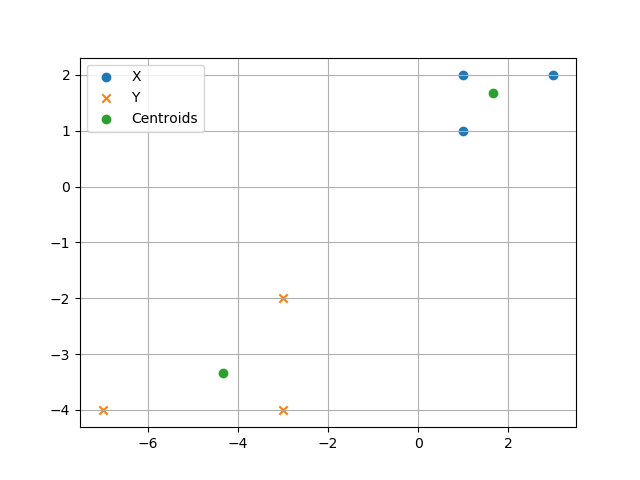
\includegraphics[width=\textwidth]{figures/procrustes_ex1}
        \caption[]
        {{\small Original coordinates}}    
        \label{fig:procrustes_ex_1}
    \end{subfigure}
    \begin{subfigure}[b]{0.475\textwidth}  
        \centering 
        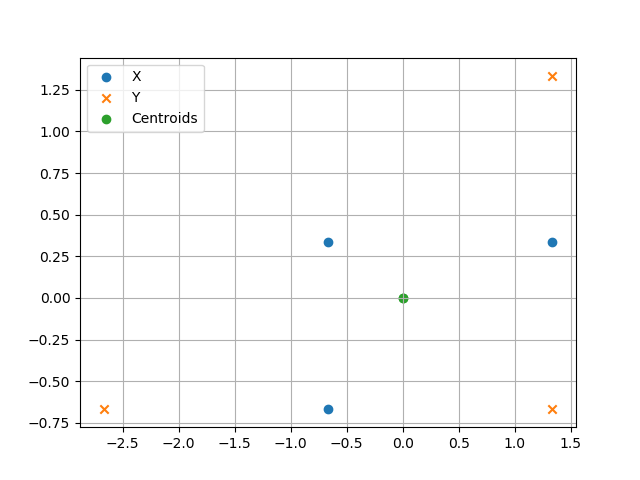
\includegraphics[width=\textwidth]{figures/procrustes_ex2}
        \caption[]
        {{\small Translation}}    
        \label{fig:procrustes_ex_2}
    \end{subfigure}
    \begin{subfigure}[b]{0.475\textwidth}   
        \centering 
        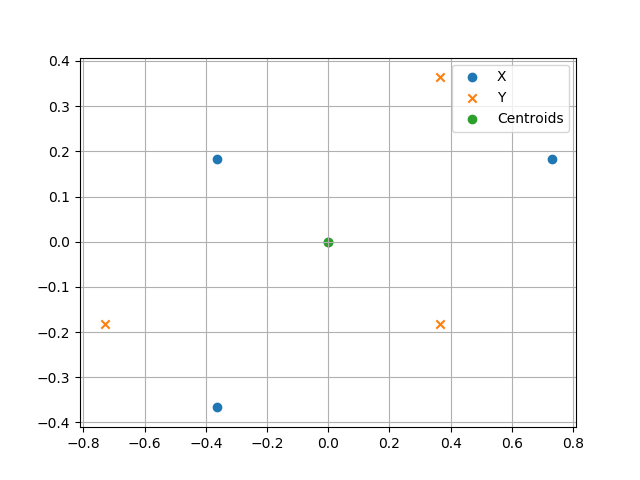
\includegraphics[width=\textwidth]{figures/procrustes_ex3}
        \caption[]
        {{\small Scaling}}    
        \label{fig:procrustes_ex_3}
    \end{subfigure}
    \begin{subfigure}[b]{0.475\textwidth}   
        \centering 
        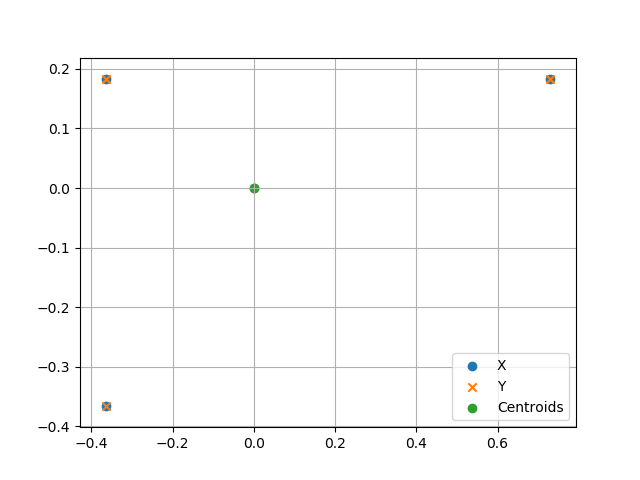
\includegraphics[width=\textwidth]{figures/procrustes_ex4}
        \caption[]
        {{\small Rotation}}    
        \label{fig:procrustes_ex_4}
    \end{subfigure}
    \caption[]
    {Application of Procrustes Analysis} 
    \label{fig:procrustes_analysis}
\end{figure*}

Before applying alignment, the sum of square differences between $\mat{X}$ and $\mat{Y}$ is
\begin{align*}
    D& = {(1+3)^2 + (1+2)^2} + {(1+3)^2 + (2+4)^2} + {(3+7)^2 + (2+4)^2} \\
     & = 213
\end{align*}
As described in section (\ref{sec:trans_align}), the initial objects are translated so that their centroids lie at the origin (Figure \ref{fig:procrustes_ex_2}). This is then followed by scaling alignment and finally rotational alignment (Figures \ref{fig:procrustes_ex_3}, \ref{fig:procrustes_ex_4}).
After alignment, the difference is zero as these objects are both similar triangles.

\subsection{Procrustes Analysis for Facial Mesh Alignment}
The process of Procrustes Analysis described above deals with objects in which all coordinate points are used to find the optimum alignment, however this is inappropriate for facial mesh alignment as not only would the position of the head be aligned to, but as would the motion from speech, of which the aim is to maintain variation.
However, a subset of points of a pair of objects can be used to align the entire object.
By selecting points which do not contain any movement due to speech or facial expression, variation in these points can be assumed to be only from head motion.
Such positions include the nose, corners of the eyes and cheekbones.
If the facial scans capture 360 degrees, then points on the back of the subjects head can also be used.
From this subset of points, the translation, scaling and rotational matrix can be found which aligns these points using the steps described in section \ref{sec:procrustes_analysis} but then applied to the entire object.
An example of such an application is shown in Figure \ref{fig:VOCASET_Alignment} before and after alignment has been applied.

%\bibliographystyle{unsrt}
%\bibliography{ref}
%\end{document}